% ============================================================
%  SENTINEL-GNSS — Individual Poster: Ingeriyinkindi Claudine (LS2525236)
%  A1 Portrait · Compile: pdflatex (single pass)
% ============================================================
\documentclass[20pt]{extarticle}
\usepackage[T1]{fontenc}
\usepackage[utf8]{inputenc}
\usepackage{lmodern}
\usepackage[a1paper,landscape=false,
            top=1.8cm,bottom=1.8cm,left=2cm,right=2cm]{geometry}
\usepackage{multicol}
\setlength{\columnsep}{1.4cm}
\usepackage{amsmath,amssymb}
\usepackage{graphicx}
\usepackage{booktabs}
\usepackage{float}
\usepackage{caption}
\captionsetup{font=large,labelfont=bf}
\usepackage[dvipsnames]{xcolor}
\definecolor{buaaBlue}{RGB}{0,91,172}
\definecolor{buaaNavy}{RGB}{0,51,102}
\definecolor{buaaSky}{RGB}{0,160,233}
\definecolor{cleanGreen}{RGB}{76,175,80}
\definecolor{degradRed}{RGB}{244,67,54}
\definecolor{blockBG}{RGB}{235,244,252}
\usepackage{tcolorbox}
\tcbuselibrary{skins}
\usepackage{mdframed}
\usepackage{parskip}
\setlength{\parskip}{5pt}
\usepackage{enumitem}
\setlist[itemize]{noitemsep,topsep=2pt}
\newmdenv[backgroundcolor=blockBG,linecolor=buaaBlue,linewidth=2pt,
          roundcorner=6pt,innertopmargin=8pt,innerbottommargin=8pt,
          innerleftmargin=10pt,innerrightmargin=10pt,
          skipabove=6pt,skipbelow=6pt]{poblock}
\newcommand{\posec}[1]{\vspace{4pt}{\large\bfseries\color{buaaNavy}#1}\\[-4pt]
  {\color{buaaBlue}\rule{\linewidth}{1.5pt}}\vspace{4pt}}
\pagestyle{empty}

\begin{document}

\noindent
\begin{tcolorbox}[colback=buaaNavy,colframe=buaaNavy,boxrule=0pt,arc=8pt,
                  left=16pt,right=16pt,top=10pt,bottom=10pt]
  \begin{center}
    {\fontsize{46}{54}\bfseries\color{white} SENTINEL-GNSS — Individual Poster}\\[6pt]
    {\fontsize{26}{32}\color{buaaSky}
     Field Data Collection, Cross-City Generalisation Testing, and Results Figures}\\[8pt]
    {\large\color{white}
     \textbf{Ingeriyinkindi Claudine} (LS2525236) \quad Field Operations \& Validation}\\[4pt]
    {\normalsize\color{white!70!buaaSky} H3I, Beihang University · Hangzhou · 2026}
  \end{center}
\end{tcolorbox}
\vspace{0.5cm}

\begin{multicols}{3}

\posec{My Role}
\begin{poblock}
I covered field operations and validation:
\begin{itemize}
  \item Campus route planning for 5 scenarios
  \item Led all 34 data collection runs (272 minutes total)
  \item Cross-geography generalisation tests (UrbanNav HK, Oxford RobotCar)
  \item Cross-city RF baseline (the 0.15 DEGRADED F1 that makes the paper)
  \item Generalisation analysis and paragraph writing
  \item 13 publication-quality figures in Matplotlib/PDF
  \item Results table formatting for Paper Section 5
\end{itemize}
\end{poblock}

\posec{Campus Data Collection}
\begin{poblock}
\textbf{Route design} — walked the campus to identify:
\begin{itemize}
  \item \textbf{Scenario A} (blockage): Library north entrance, 100\,m open approach
  \item \textbf{Scenario B} (urban canyon): Student Centre east corridor, 300\,m
  \item \textbf{Scenario C} (canopy): Dormitory avenue, dense tree cover
  \item \textbf{Scenario D} (open sky): East sports ground, 360° horizon
  \item \textbf{Scenario E} (gradual): 3 building faces, 5 reps each
\end{itemize}

\textbf{Collection protocol:}
Start 2\,min before moving · log blockage times · Joshua verifies on-site.
\end{poblock}

\begin{center}
  \begin{tabular}{lcccc}
    \toprule
    Scenario & Runs & DEG epochs & CLEAN epochs \\
    \midrule
    A & 10 & 820 & 1,240 \\
    B & 5  & 480 & 380   \\
    C & 3  & 260 & 2,100 \\
    D & 1  & 0   & 1,920 \\
    E & 15 & 1,140 & 2,350 \\
    \midrule
    \textbf{Total} & \textbf{34} & \textbf{2,700} & \textbf{7,990} \\
    \bottomrule
  \end{tabular}
\end{center}

\posec{Cross-Geography Generalisation Testing}
\begin{poblock}
I applied the trained SENTINEL model (\textbf{no retraining}) to:
\begin{enumerate}
  \item UrbanNav HK Medium, Deep, Harsh, Tunnel
  \item Oxford RobotCar GNSS
  \item \textbf{UrbanNav Tokyo} (held-out test city)
\end{enumerate}

\textbf{Critical methodology:} Used the \emph{same} normalisation parameters
from Beihang training data — never refit to evaluation city.
Re-fitting would inflate performance by 5–10\,\%.
\end{poblock}

\posec{The Central Cross-City Result}
\begin{poblock}
\begin{tabular}{lcc}
  \toprule
  Model & Tokyo Macro-F1 & Tokyo DEG F1 \\
  \midrule
  \textbf{SENTINEL (DL)} & 0.649 & \textbf{\textcolor{cleanGreen}{0.753}} \\
  RandomForest           & 0.618 & \textbf{\textcolor{degradRed}{0.148}} \\
  \bottomrule
\end{tabular}

\medskip
\textbf{5$\times$ gap in safety-critical DEGRADED F1.}

\medskip
I ran the RF evaluation myself to confirm it was not an artifact.
The RF memorises Beihang-specific C/N$_0$ thresholds.
Tokyo's Shinjuku district has different mean C/N$_0$ (taller buildings,
different satellite elevation cutoffs) → RF mis-classifies systematically.

\medskip
\textbf{Surprising finding:} Tokyo DEGRADED F1 (0.753) $>$ UrbanNav HK Deep (0.687).
Shinjuku's regular skyscraper geometry creates cleaner NLOS transitions than
Hong Kong's irregular canyons. I wrote this interpretation.
\end{poblock}

\begin{center}
  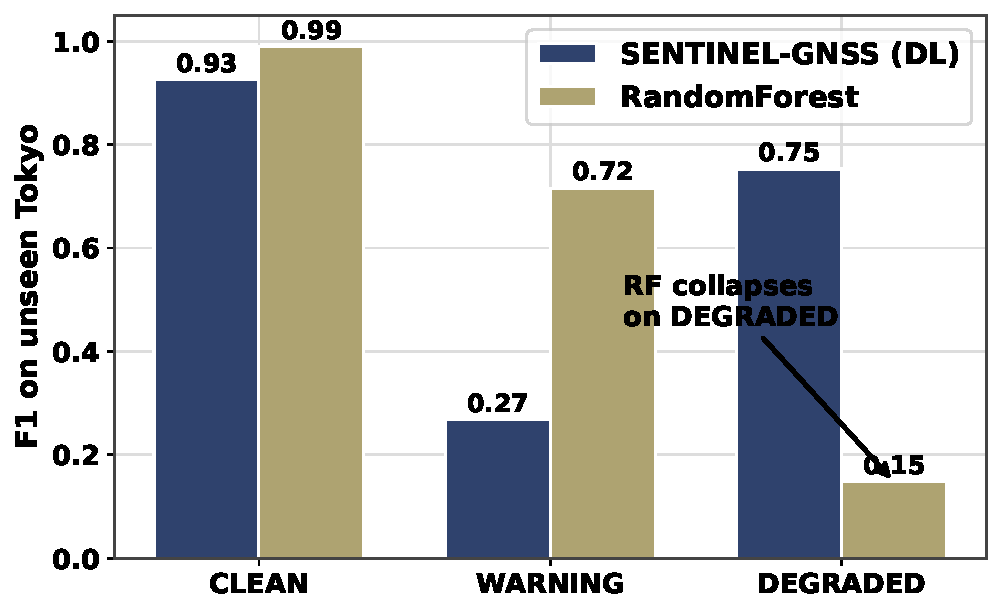
\includegraphics[width=0.9\columnwidth]{../../results/paper_figures/fig05_crosscity_degraded.pdf}
  \captionof{figure}{DEGRADED F1 cross-city: DL transfers, RF collapses.}
\end{center}

\begin{center}
  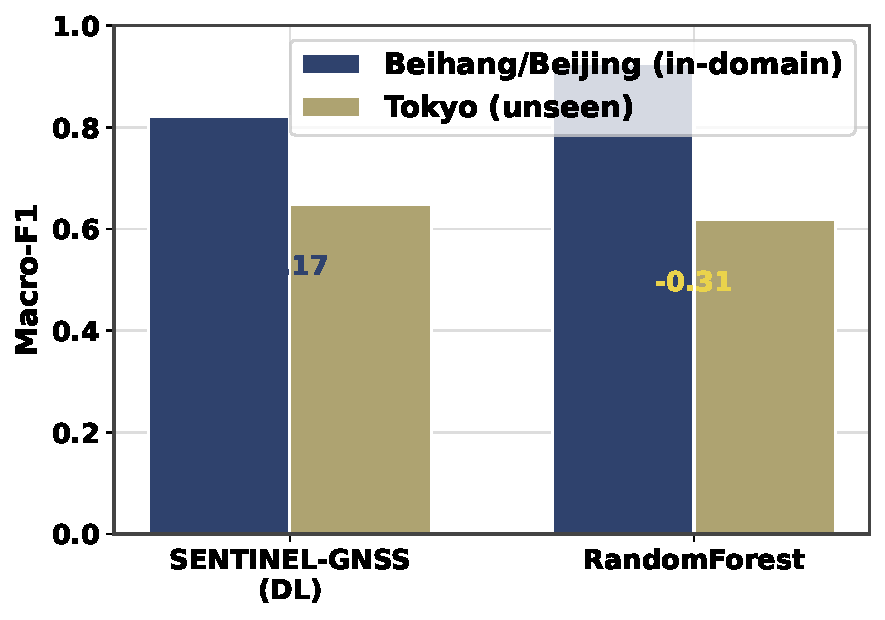
\includegraphics[width=0.85\columnwidth]{../../results/paper_figures/fig06_crosscity_gap.pdf}
  \captionof{figure}{Cross-city Macro-F1 gap. DL gap ($-$0.17) vs RF ($-$0.31).}
\end{center}

\posec{Publication Figures I Produced}
\begin{poblock}
\begin{tabular}{lp{6cm}}
  \toprule
  Figure & Content \\
  \midrule
  \texttt{multi\_horizon\_comparison} & Macro-F1 all horizons \\
  \texttt{confusion\_matrices\_test}  & 3-panel confusion matrices \\
  \texttt{pr\_curves\_test}           & Precision-recall curves \\
  \texttt{roc\_curves\_test}          & ROC with AUC \\
  \texttt{lead\_time\_histogram}      & Advance warning seconds \\
  \texttt{learning\_curves}           & Train/val F1 vs epoch \\
  \texttt{attention\_heatmap\_*}      & Transformer attention \\
  \texttt{feature\_saliency\_*}       & Permutation importance \\
  \bottomrule
\end{tabular}

\medskip
Style: Beihang palette · 12pt minimum axis labels · 300\,dpi PNG + PDF vector
\end{poblock}

\begin{center}
  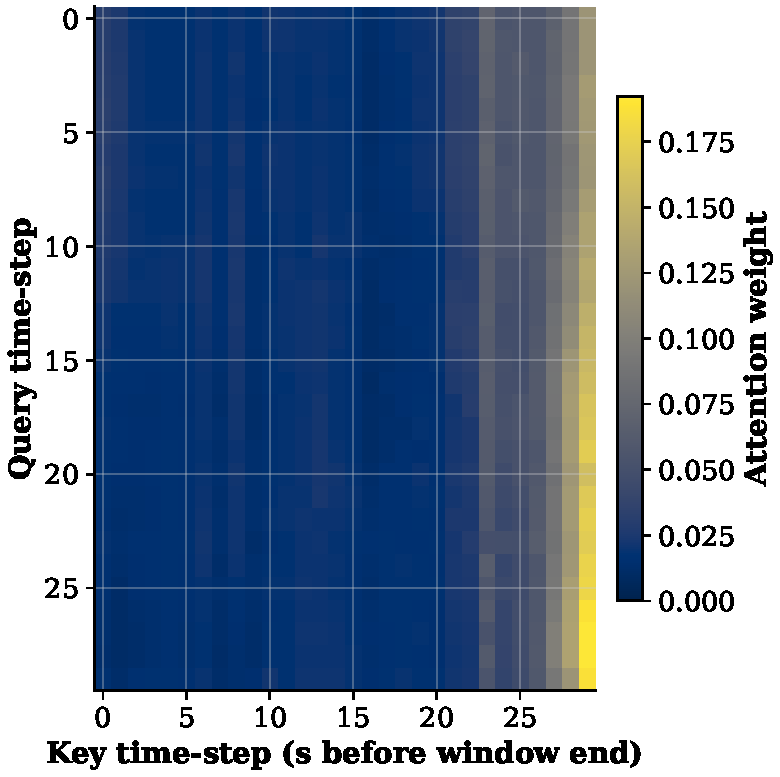
\includegraphics[width=0.88\columnwidth]{../../results/paper_figures/attention_heatmap_degraded.pdf}
  \captionof{figure}{Transformer attention for DEGRADED prediction: strongest
  attention on the 5–15 epochs before the prediction window.}
\end{center}

\posec{Key Lesson}
\begin{poblock}
\textbf{Cross-city evaluation is the decisive test, not in-domain leaderboard rank.}
A classifier that achieves 0.93 Macro-F1 in-domain but collapses to 0.15
DEGRADED F1 on an unseen city is not deployable.
The 5$\times$ gap I measured is what makes SENTINEL's contribution real.

\medskip
\textbf{Collection lesson:} A live SNR display during collection would
have saved 4 discarded runs. GNSS signal health should be monitored
in real time during field data collection, not discovered post-processing.
\end{poblock}

\end{multicols}

\noindent{\color{buaaBlue}\rule{\linewidth}{1.5pt}}\\[2pt]
{\small\color{buaaNavy}\centering H3I, Beihang University · Hangzhou · 2026}

\end{document}
